% Unidad 0. Herramientas matemáticas para Física y Química
%----------------------------------------------------------------------------------------
% A. Las destrezas científicas básicas
%   - Herramientas matemáticas básicas en diferentes escenarios científicos: potencias de 10
%     (significado, paso a decimal, multiplicación, división, cambio de lado de la raya de
%     fracción y potencia de una potencia), despeje de ecuaciones de primer grado (método de
%     operar en los dos miembros y método de "pasar" al otro lado, incógnita en el
%     denominador) y representación e interpretación de gráficas lineales (ejes con nombre de
%     magnitudes, "A frente a B", pendiente y ordenada en el origen).
%
% Unidad de repaso: se trabaja como Unidad 0, antes de empezar las unidades de Química y Física.
% Traducción al español de MathTools.tex.
%----------------------------------------------------------------------------------------

\spacing{1.3}
\raggedbottom % pages with large figures end where the text ends (no stretched gaps between boxes)

En física y química usamos las matemáticas continuamente: para escribir números muy grandes y muy pequeños, para calcular una magnitud a partir de una fórmula o para dibujar e interpretar gráficas. Esta unidad es una \textbf{caja de herramientas}: puedes volver a ella siempre que necesites recordar cómo se hace algo.

%----------------------------------------------------------------------------------------

\section{Potencias de 10}

\subsection{¿Qué es una potencia de 10?}

\begin{definition}[Potencia de 10]
    Es un número de la forma \(10^{n}\), donde el \textbf{exponente} \(n\) es un número entero. Significa que multiplicamos el 10 por sí mismo \(n\) veces: \(10^{3} = 10 \cdot 10 \cdot 10 = 1000\).
\end{definition}

\begin{figure}[H]
    \centering
    % [FIGURA ORIGINAL] \includegraphics[width=\textwidth]{Unit_0/power10_line}
    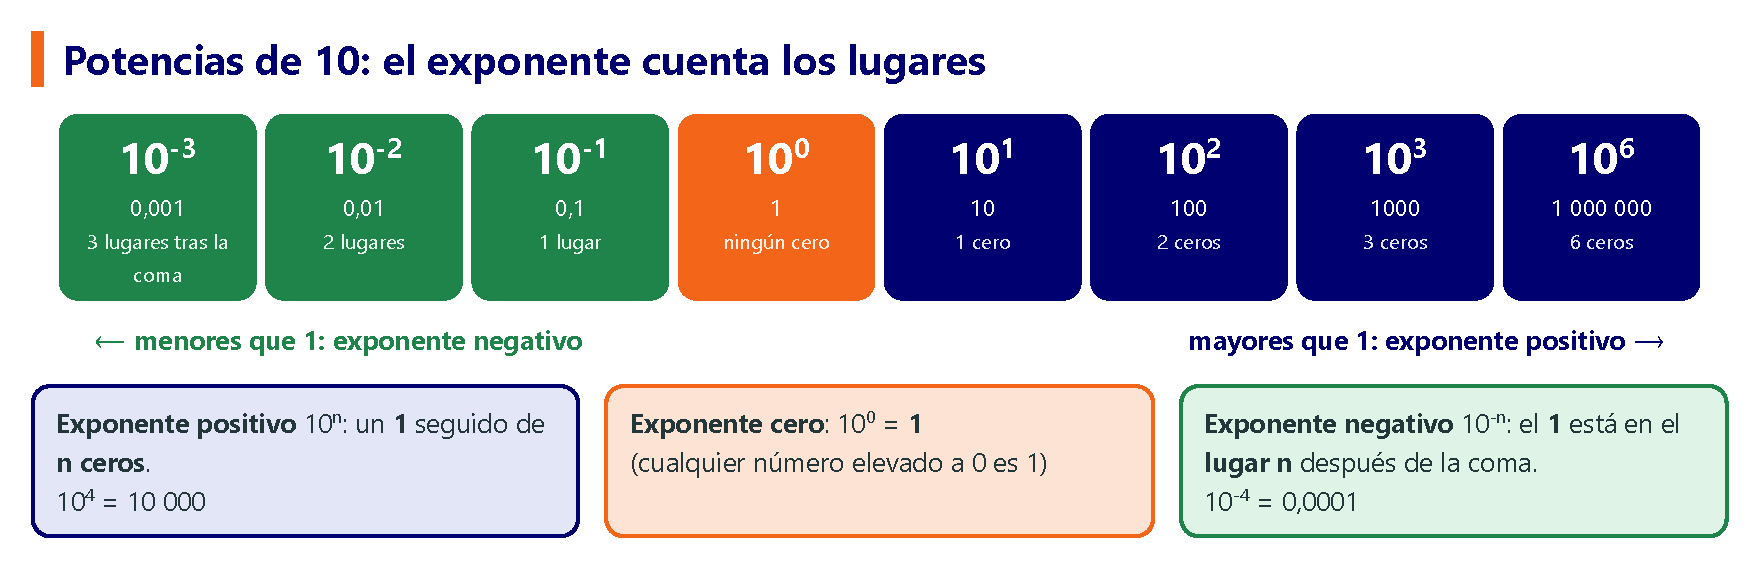
\includegraphics[width=\textwidth]{FigurasSVG/Unit_0_Math_Tools/pdf/power10_line_es.pdf}
    \caption{Los exponentes positivos dan números mayores que 1; los exponentes negativos dan números menores que 1.}
    \label{fig:u0_power10_line}
\end{figure}

\begin{impt}
    \begin{itemize}
        \item \(10^{n}\) con \(n\) \textbf{positivo}: un \textbf{1} seguido de \textbf{\(n\) ceros}. \quad \(10^{5} = \num{100000}\).
        \item \(10^{0} = 1\).
        \item \(10^{-n}\) con \(n\) \textbf{positivo}: un número decimal con el \textbf{1} en el \textbf{lugar \(n\)} después de la coma. \quad \(10^{-5} = \num{0.00001}\).
    \end{itemize}
\end{impt}

\subsection{Escribir números con potencias de 10, y volver a decimal}

Cualquier número se puede escribir como un número multiplicado por una potencia de 10. Sigue siendo \textbf{el mismo número}, solo que escrito de otra forma:
\begin{equation*}
    \num{5000} = 5 \cdot \num{1000} = 5 \cdot 10^{3}
    \qquad\qquad
    \num{0.007} = 7 \cdot \num{0.001} = 7 \cdot 10^{-3}
\end{equation*}

\negsubro{De potencia de 10 a número decimal}: el exponente nos dice cuántos lugares se mueve la coma.
\begin{itemize}
    \item Exponente \textbf{positivo}: la coma se mueve hacia la \textbf{derecha} (el número se hace más grande). Si no quedan más cifras, añadimos ceros: \(\num{3.2e4} = 3{,}2 \to 32\,000\).
    \item Exponente \textbf{negativo}: la coma se mueve hacia la \textbf{izquierda} (el número se hace más pequeño). Si no quedan más cifras, añadimos ceros y un 0 delante de la coma: \(\num{4.5e-3} = \num{0.0045}\).
\end{itemize}

\begin{example}
    \textbf{Escribe como potencia de 10 y después vuelve a escribirlo en forma decimal.}
    \begin{itemize}
        \item \(\num{1000000} = 10^{6}\) (un 1 y seis ceros). Vuelta: \(10^{6}\) \(\to\) un 1 seguido de 6 ceros \(= \num{1000000}\).
        \item \(\num{0.01} = 10^{-2}\) (el 1 está en el 2.º lugar después de la coma). Vuelta: \(10^{-2} = \num{0.01}\).
        \item \(\num{80000} = 8 \cdot 10^{4}\). Vuelta: \(8 \cdot 10^{4}\) \(\to\) la coma del 8 se mueve 4 lugares a la derecha: \(\num{80000}\).
        \item \(\num{0.0006} = 6 \cdot 10^{-4}\). Vuelta: \(6 \cdot 10^{-4}\) \(\to\) la coma del 6 se mueve 4 lugares a la izquierda: \(\num{0.0006}\).
    \end{itemize}
\end{example}

\begin{exercise}
    Escribe estos números como una potencia de 10 (o como un número por una potencia de 10):
    \begin{enumerate}[label=\letraminuscula]
        \item \num{10000}
        \item \num{0.001}
        \item \num{100000000}
        \item \num{0.000001}
        \item \num{3000}
        \item \num{0.05}
        \item \num{7000000}
        \item \num{0.0009}
    \end{enumerate}
    \begin{solu}
        a) \(10^{4}\); b) \(10^{-3}\); c) \(10^{8}\); d) \(10^{-6}\); e) \(3 \cdot 10^{3}\); f) \(5 \cdot 10^{-2}\); g) \(7 \cdot 10^{6}\); h) \(9 \cdot 10^{-4}\).
    \end{solu}
\end{exercise}

\begin{exercise}
    Escribe estos números en forma decimal:
    \begin{enumerate}[label=\letraminuscula]
        \item \(10^{3}\)
        \item \(10^{-4}\)
        \item \(2 \cdot 10^{5}\)
        \item \(6{,}5 \cdot 10^{2}\)
        \item \(3 \cdot 10^{-2}\)
        \item \(1{,}2 \cdot 10^{-3}\)
    \end{enumerate}
    \begin{solu}
        a) \num{1000}; b) \num{0.0001}; c) \num{200000}; d) \num{650}; e) \num{0.03}; f) \num{0.0012}.
    \end{solu}
\end{exercise}

\subsection{Las reglas de las potencias de 10}

\begin{figure}[H]
    \centering
    % [FIGURA ORIGINAL] \includegraphics[width=\textwidth]{Unit_0/power10_rules}
    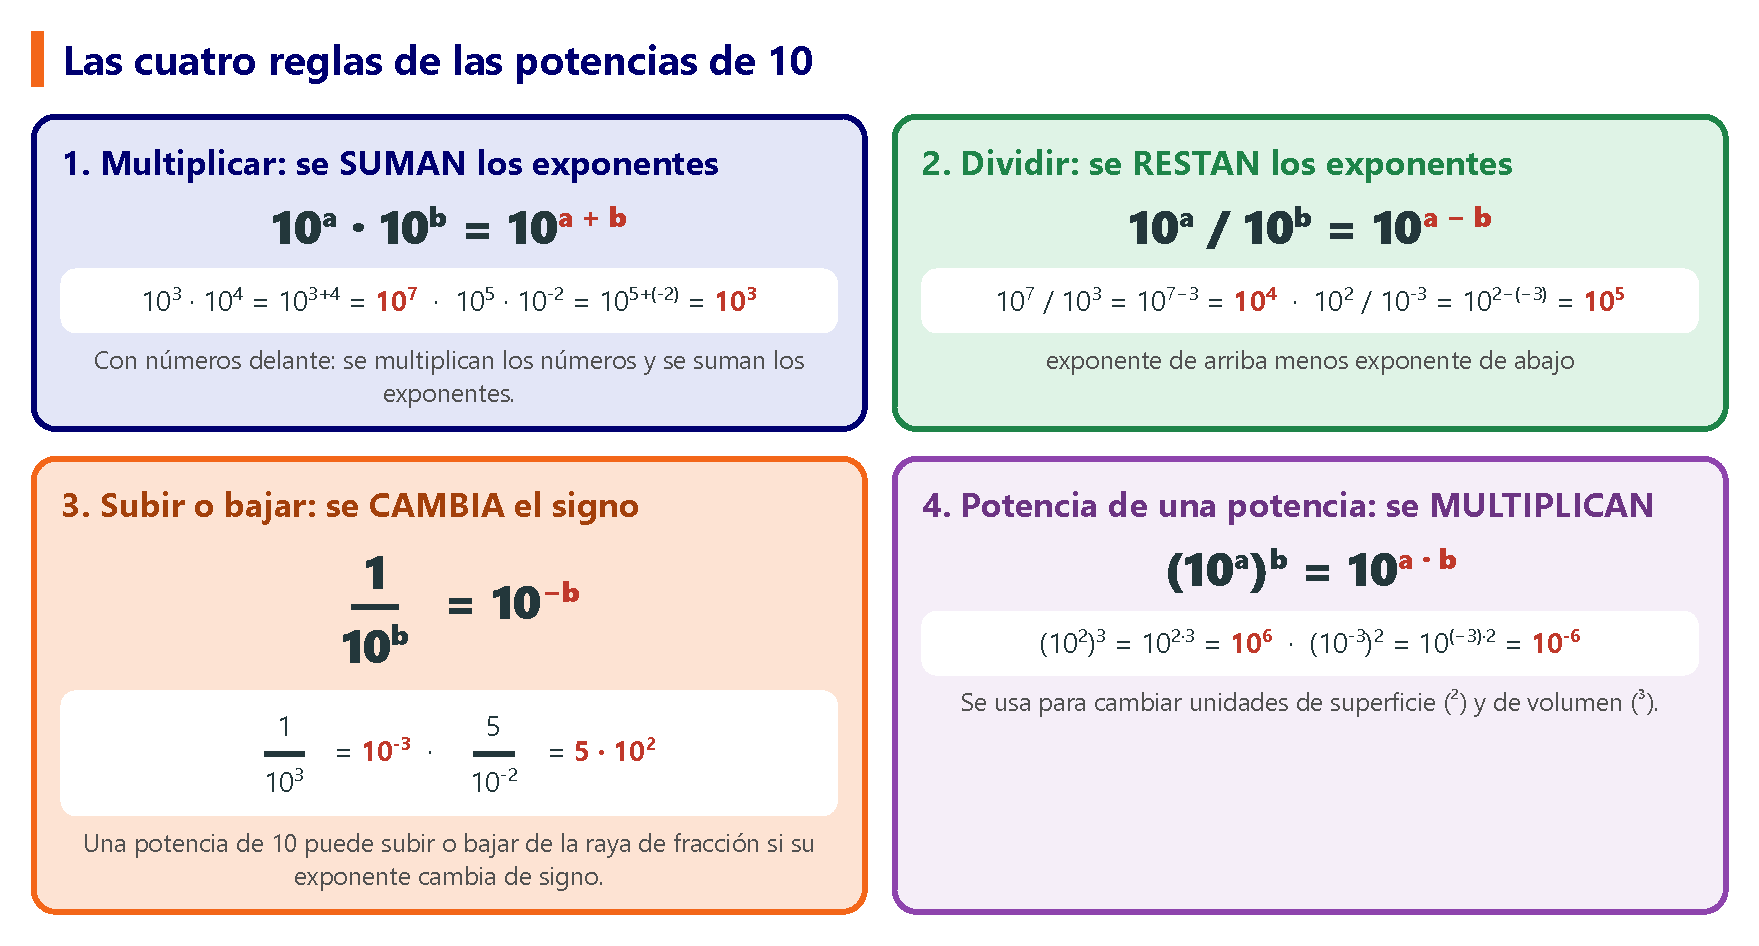
\includegraphics[width=\textwidth]{FigurasSVG/Unit_0_Math_Tools/pdf/power10_rules_es.pdf}
    \caption{Las cuatro reglas para operar con potencias de 10.}
    \label{fig:u0_power10_rules}
\end{figure}

\subsubsection{Multiplicar: se suman los exponentes}

\begin{equation*}
    10^{a} \cdot 10^{b} = 10^{a+b}
\end{equation*}

Si las potencias de 10 llevan un número delante, multiplicamos por un lado los números y por otro las potencias de 10:

\begin{example}
    \begin{itemize}
        \item \(10^{3} \cdot 10^{5} = 10^{3+5} = \textcolor{red}{10^{8}}\)
        \item \(10^{6} \cdot 10^{-2} = 10^{6+(-2)} = \textcolor{red}{10^{4}}\)
        \item \((3 \cdot 10^{4}) \cdot (2 \cdot 10^{3}) = (3 \cdot 2) \cdot 10^{4+3} = \textcolor{red}{6 \cdot 10^{7}}\)
        \item \((5 \cdot 10^{-3}) \cdot (4 \cdot 10^{6}) = 20 \cdot 10^{3} = \textcolor{red}{2 \cdot 10^{4}}\)
    \end{itemize}
\end{example}

\subsubsection{Dividir: se restan los exponentes}

\begin{equation*}
    \dfrac{10^{a}}{10^{b}} = 10^{a-b}
\end{equation*}

Restamos: exponente de arriba \textbf{menos} exponente de abajo. ¡Cuidado con los signos!

\begin{example}
    \begin{itemize}
        \item \(\dfrac{10^{8}}{10^{3}} = 10^{8-3} = \textcolor{red}{10^{5}}\)
        \item \(\dfrac{10^{2}}{10^{-4}} = 10^{2-(-4)} = 10^{2+4} = \textcolor{red}{10^{6}}\)
        \item \(\dfrac{8 \cdot 10^{6}}{2 \cdot 10^{2}} = \dfrac{8}{2} \cdot 10^{6-2} = \textcolor{red}{4 \cdot 10^{4}}\)
        \item \(\dfrac{9 \cdot 10^{-3}}{3 \cdot 10^{2}} = 3 \cdot 10^{-3-2} = \textcolor{red}{3 \cdot 10^{-5}}\)
    \end{itemize}
\end{example}

\subsubsection{Subir o bajar una potencia de 10: se cambia el signo del exponente}

Una potencia de 10 que está \textbf{debajo} de la raya de fracción se puede pasar \textbf{arriba} (y al revés) si \textbf{cambiamos el signo} de su exponente:
\begin{equation*}
    \dfrac{1}{10^{b}} = 10^{-b}
    \qquad\qquad
    10^{-b} = \dfrac{1}{10^{b}}
\end{equation*}

\begin{figure}[H]
    \centering
    % [FIGURA ORIGINAL] \includegraphics[width=\textwidth]{Unit_0/power10_flip}
    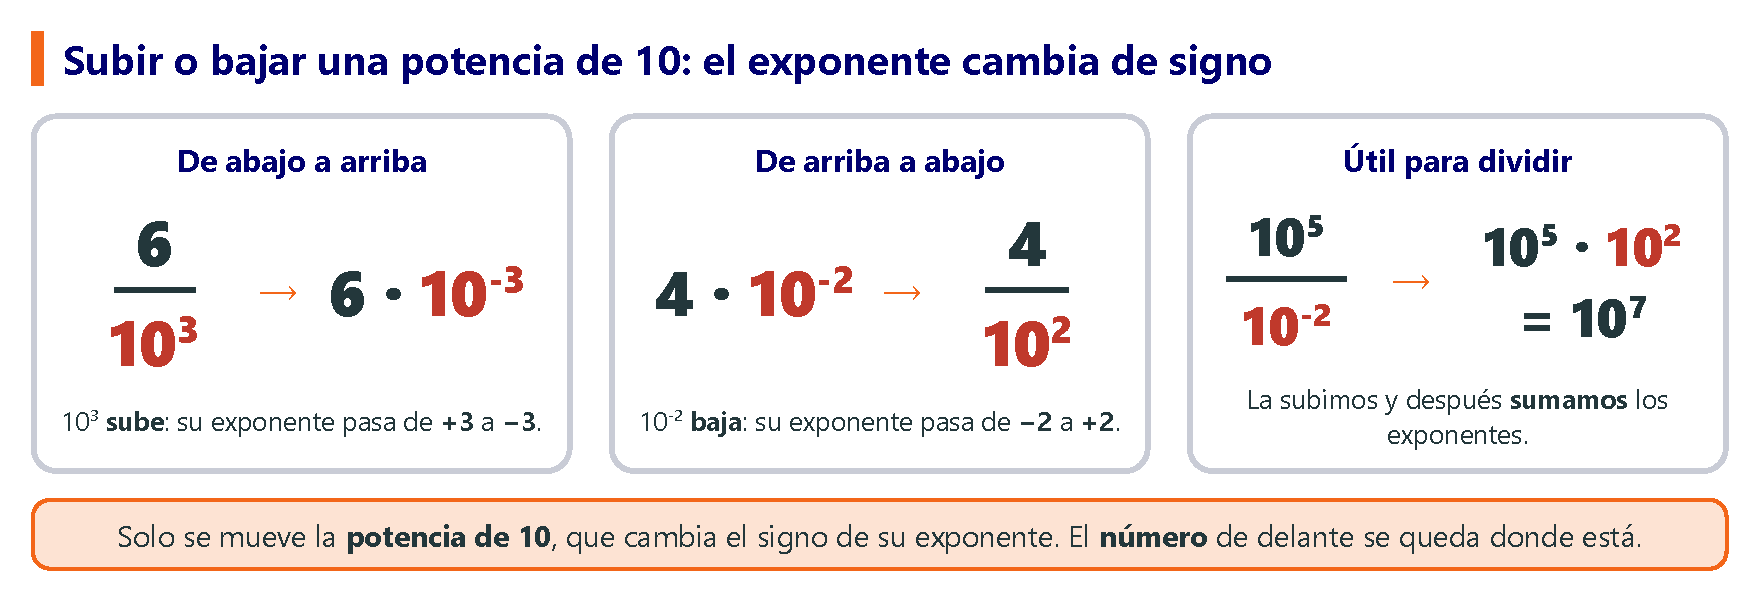
\includegraphics[width=\textwidth]{FigurasSVG/Unit_0_Math_Tools/pdf/power10_flip_es.pdf}
    \caption{Cuando una potencia de 10 cruza la raya de fracción, su exponente cambia de signo.}
    \label{fig:u0_power10_flip}
\end{figure}

\begin{example}
    \begin{itemize}
        \item \(\dfrac{6}{10^{3}} = \textcolor{red}{6 \cdot 10^{-3}}\) \quad (\(10^{3}\) sube como \(10^{-3}\))
        \item \(\dfrac{7}{10^{-2}} = \textcolor{red}{7 \cdot 10^{2}}\) \quad (\(10^{-2}\) sube como \(10^{2}\))
        \item \(\dfrac{10^{5}}{10^{-2}} = 10^{5} \cdot 10^{2} = \textcolor{red}{10^{7}}\) \quad (la subimos y después sumamos los exponentes; es el mismo resultado que restar \(5 - (-2) = 7\))
        \item Esto es muy útil con los factores de conversión: \(\num{450}\,\unit{\mg} \cdot \dfrac{\qty{1}{\g}}{\qty{e3}{\mg}} = 450 \cdot 10^{-3}\,\unit{\g} = \qty{0.45}{\g}\).
    \end{itemize}
\end{example}

\subsubsection{Potencia de una potencia: se multiplican los exponentes}

\begin{equation*}
    \left(10^{a}\right)^{b} = 10^{a \cdot b}
\end{equation*}

Si hay un número delante, también se eleva a la potencia: \(\left(3 \cdot 10^{2}\right)^{2} = 3^{2} \cdot 10^{2 \cdot 2} = 9 \cdot 10^{4}\).

\begin{example}
    \begin{itemize}
        \item \(\left(10^{3}\right)^{2} = 10^{3 \cdot 2} = \textcolor{red}{10^{6}}\)
        \item \(\left(10^{-2}\right)^{3} = 10^{(-2) \cdot 3} = \textcolor{red}{10^{-6}}\)
        \item \(\left(2 \cdot 10^{4}\right)^{3} = 2^{3} \cdot 10^{4 \cdot 3} = \textcolor{red}{8 \cdot 10^{12}}\)
        \item Es lo que hacemos al cambiar unidades de volumen: \(\left(\dfrac{\qty{e2}{\cm}}{\qty{1}{\m}}\right)^{3} = \dfrac{10^{2 \cdot 3}\,\unit{\cubic\cm}}{\qty{1}{\cubic\m}} = \dfrac{\qty{e6}{\cubic\cm}}{\qty{1}{\cubic\m}}\).
    \end{itemize}
\end{example}

\begin{exercise}
    \textbf{Multiplicar.} Calcula y deja el resultado como potencia de 10:
    \begin{enumerate}[label=\letraminuscula]
        \item \(10^{4} \cdot 10^{2}\)
        \item \(10^{-3} \cdot 10^{-5}\)
        \item \(10^{7} \cdot 10^{-4}\)
        \item \((2 \cdot 10^{3}) \cdot (4 \cdot 10^{5})\)
        \item \((3 \cdot 10^{-2}) \cdot (3 \cdot 10^{6})\)
        \item \((5 \cdot 10^{4}) \cdot (6 \cdot 10^{-7})\)
    \end{enumerate}
    \begin{solu}
        a) \(10^{6}\); b) \(10^{-8}\); c) \(10^{3}\); d) \(8 \cdot 10^{8}\); e) \(9 \cdot 10^{4}\); f) \(30 \cdot 10^{-3} = 3 \cdot 10^{-2}\).
    \end{solu}
\end{exercise}

\begin{exercise}
    \textbf{Dividir.} Calcula y deja el resultado como potencia de 10:
    \begin{enumerate}[label=\letraminuscula]
        \item \(\dfrac{10^{9}}{10^{4}}\)
        \item \(\dfrac{10^{3}}{10^{-2}}\)
        \item \(\dfrac{10^{-4}}{10^{2}}\)
        \item \(\dfrac{6 \cdot 10^{8}}{3 \cdot 10^{5}}\)
        \item \(\dfrac{8 \cdot 10^{-2}}{4 \cdot 10^{-6}}\)
        \item \(\dfrac{12 \cdot 10^{3}}{4 \cdot 10^{7}}\)
    \end{enumerate}
    \begin{solu}
        a) \(10^{5}\); b) \(10^{5}\); c) \(10^{-6}\); d) \(2 \cdot 10^{3}\); e) \(2 \cdot 10^{4}\); f) \(3 \cdot 10^{-4}\).
    \end{solu}
\end{exercise}

\begin{exercise}
    \textbf{Subir.} Escribe sin fracciones, pasando la potencia de 10 arriba:
    \begin{enumerate}[label=\letraminuscula]
        \item \(\dfrac{1}{10^{4}}\)
        \item \(\dfrac{3}{10^{2}}\)
        \item \(\dfrac{5}{10^{-3}}\)
        \item \(\dfrac{10^{2}}{10^{-5}}\)
    \end{enumerate}
    \begin{solu}
        a) \(10^{-4}\); b) \(3 \cdot 10^{-2}\); c) \(5 \cdot 10^{3}\); d) \(10^{2} \cdot 10^{5} = 10^{7}\).
    \end{solu}
\end{exercise}

\begin{exercise}
    \textbf{Potencia de una potencia.} Calcula:
    \begin{enumerate}[label=\letraminuscula]
        \item \(\left(10^{4}\right)^{2}\)
        \item \(\left(10^{-1}\right)^{3}\)
        \item \(\left(10^{-3}\right)^{-2}\)
        \item \(\left(3 \cdot 10^{2}\right)^{3}\)
        \item \(\left(\dfrac{\qty{e3}{\mm}}{\qty{1}{\m}}\right)^{2}\)
    \end{enumerate}
    \begin{solu}
        a) \(10^{8}\); b) \(10^{-3}\); c) \(10^{6}\); d) \(27 \cdot 10^{6} = 2{,}7 \cdot 10^{7}\); e) \(\dfrac{\qty{e6}{\square\mm}}{\qty{1}{\square\m}}\).
    \end{solu}
\end{exercise}

\begin{exercise}
    \textbf{Mezcla.} Calcula, dejando el resultado como potencia de 10, y después escríbelo en forma decimal:
    \begin{enumerate}[label=\letraminuscula]
        \item \(\dfrac{10^{3} \cdot 10^{4}}{10^{5}}\)
        \item \(\dfrac{10^{-2} \cdot 10^{6}}{10^{-1}}\)
        \item \(\dfrac{(2 \cdot 10^{3})^{2}}{4 \cdot 10^{2}}\)
    \end{enumerate}
    \begin{solu}
        a) \(\dfrac{10^{7}}{10^{5}} = 10^{2} = 100\); \quad
        b) \(\dfrac{10^{4}}{10^{-1}} = 10^{5} = \num{100000}\); \quad
        c) \(\dfrac{4 \cdot 10^{6}}{4 \cdot 10^{2}} = 10^{4} = \num{10000}\).
    \end{solu}
\end{exercise}

%----------------------------------------------------------------------------------------

\section{Ecuaciones: cómo despejar una magnitud}

\subsection{¿Qué significa despejar?}

En ciencias, las fórmulas relacionan varias magnitudes: \(d = \dfrac{m}{V}\), \(v = \dfrac{x}{t}\), \(F = m \cdot a\)\ldots{} Muchas veces conocemos algunas de ellas y queremos calcular otra que no está sola. Entonces tenemos que \textbf{despejarla}.

\begin{definition}[Despejar una magnitud]
    \textbf{Despejar} una magnitud es reorganizar una ecuación para que esa magnitud quede \textbf{completamente sola} en un lado del signo igual, \textbf{en el numerador}, y todo lo demás quede en el otro lado.
\end{definition}

\begin{figure}[H]
    \centering
    % [FIGURA ORIGINAL] \includegraphics[width=\textwidth]{Unit_0/isolate_meaning}
    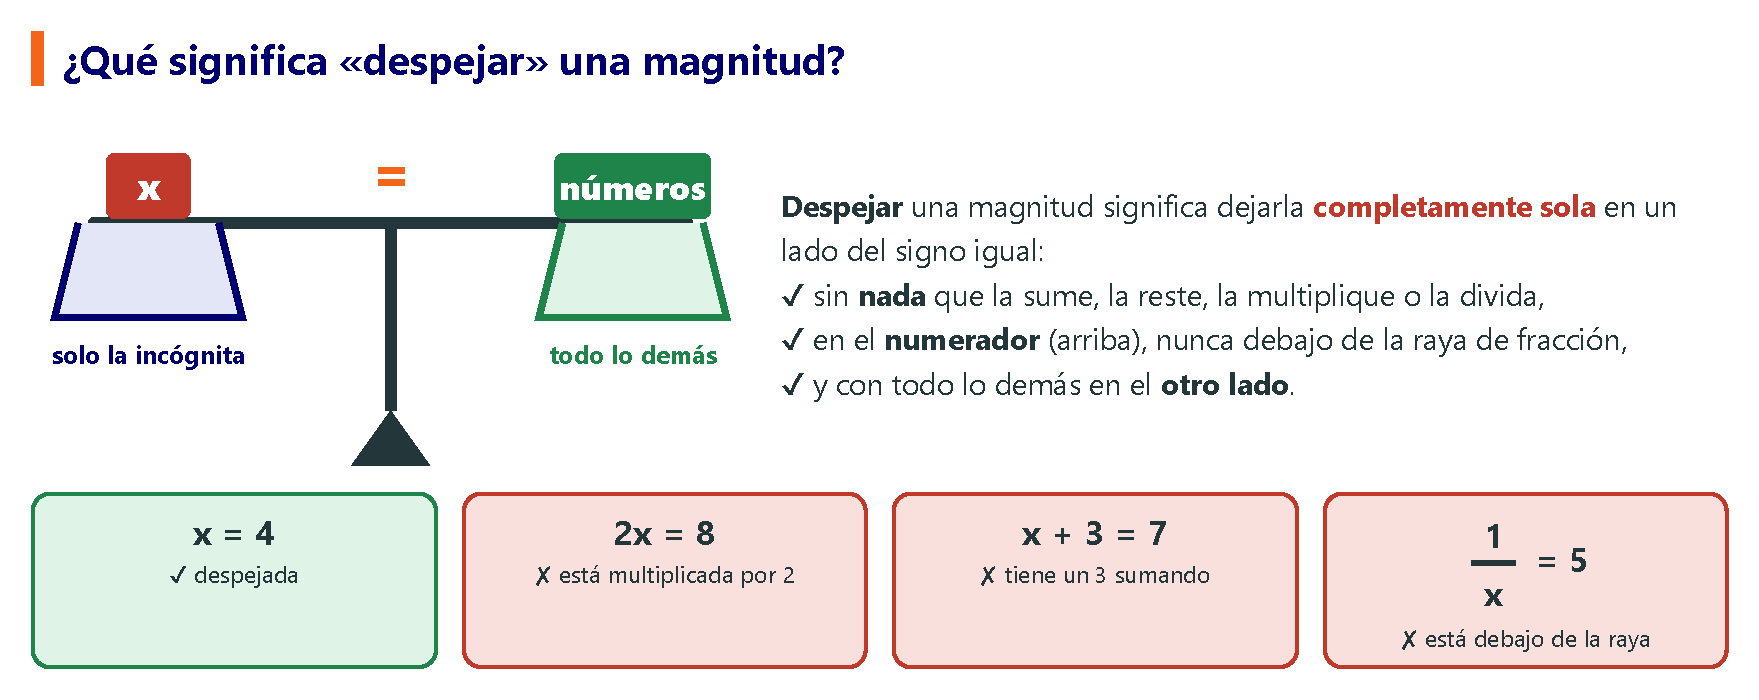
\includegraphics[width=\textwidth]{FigurasSVG/Unit_0_Math_Tools/pdf/isolate_meaning_es.pdf}
    \caption{Una ecuación es como una balanza equilibrada. Despejar es dejar la incógnita sola en uno de los lados.}
    \label{fig:u0_isolate_meaning}
\end{figure}

Una ecuación es como una \textbf{balanza equilibrada}: los dos lados (los dos \textbf{miembros}) son iguales. Si hacemos la \textbf{misma operación en los dos miembros}, la balanza sigue equilibrada y la ecuación sigue siendo cierta. Usamos esto para quitar, una a una, todas las cosas que acompañan a la incógnita.

\subsection{Dos métodos para despejar}

\begin{figure}[H]
    \centering
    % [FIGURA ORIGINAL] \includegraphics[width=\textwidth]{Unit_0/isolate_shortcut}
    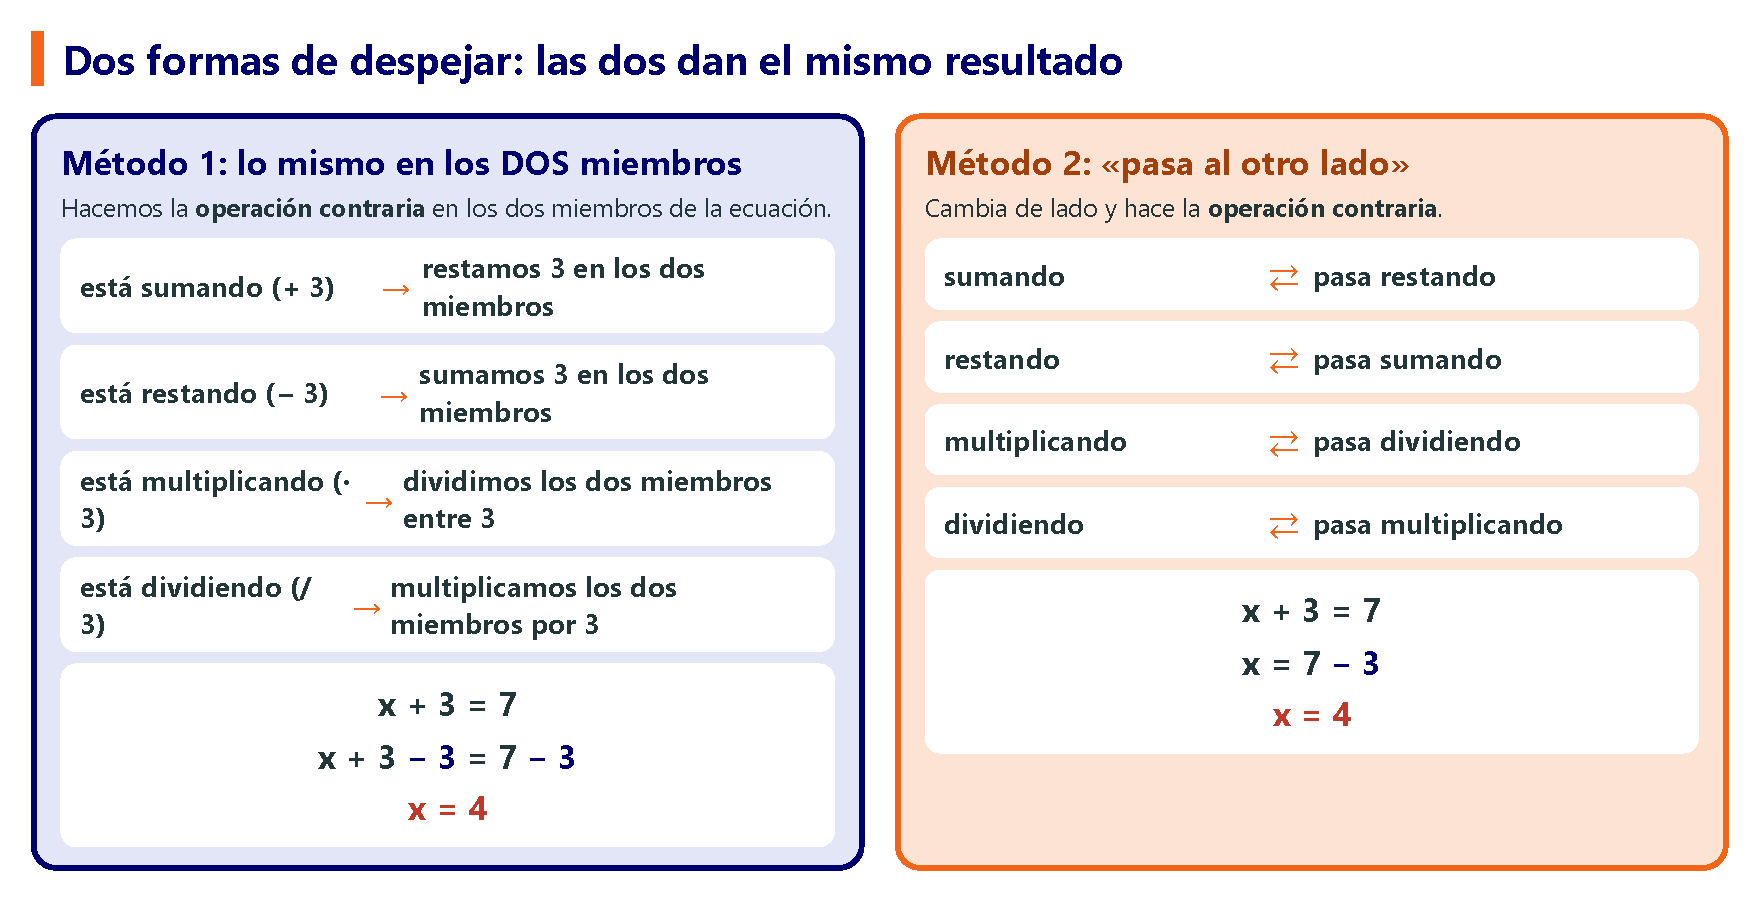
\includegraphics[width=\textwidth]{FigurasSVG/Unit_0_Math_Tools/pdf/isolate_shortcut_es.pdf}
    \caption{El método 1 (la misma operación en los dos miembros) y el método 2 (pasar al otro lado) dan el mismo resultado.}
    \label{fig:u0_isolate_shortcut}
\end{figure}

\negsubro{Método 1: la misma operación en los dos miembros} (el método de las matemáticas). Miramos qué está «pegado» a la incógnita y hacemos la \textbf{operación contraria en los dos miembros}:
\begin{itemize}
    \item Si está \textbf{sumando}, lo \textbf{restamos} en los dos miembros.
    \item Si está \textbf{restando}, lo \textbf{sumamos} en los dos miembros.
    \item Si está \textbf{multiplicando}, \textbf{dividimos} los dos miembros entre él.
    \item Si está \textbf{dividiendo}, \textbf{multiplicamos} los dos miembros por él.
\end{itemize}

\negsubro{Método 2: pasar al otro lado} (el atajo). Una cantidad puede \textbf{cambiar de lado} si también \textbf{cambia su operación} por la contraria:
\begin{center}
    \renewcommand{\arraystretch}{1.3}
    \begin{tabular}{ccc}
        \toprule
        \textbf{Si está\ldots} & & \textbf{pasa al otro lado\ldots} \\
        \midrule
        sumando \((+)\) & \(\longleftrightarrow\) & restando \((-)\) \\
        restando \((-)\) & \(\longleftrightarrow\) & sumando \((+)\) \\
        multiplicando \((\cdot)\) & \(\longleftrightarrow\) & dividiendo \((/)\) \\
        dividiendo \((/)\) & \(\longleftrightarrow\) & multiplicando \((\cdot)\) \\
        \bottomrule
    \end{tabular}
\end{center}

\begin{impt}
    El método 2 es solo una forma rápida de escribir el método 1: cuando «pasamos» el 3 restando, en realidad estamos restando 3 en los dos miembros. Usa el método que mejor entiendas, pero ¡\textbf{nunca} cambies la operación sin cambiar de lado!
\end{impt}

\subsection{Ejemplos con los dos métodos}

\begin{example}
    \textbf{Sumando: \(x + 5 = 12\).}
    \begin{itemize}
        \item Método 1: restamos 5 en los dos miembros: \(x + 5 \textcolor{blue}{- 5} = 12 \textcolor{blue}{- 5}\) \(\Rightarrow\) \(\textcolor{red}{x = 7}\).
        \item Método 2: el 5 está sumando, así que pasa al otro lado restando: \(x = 12 - 5\) \(\Rightarrow\) \(\textcolor{red}{x = 7}\).
    \end{itemize}
\end{example}

\begin{example}
    \textbf{Restando: \(x - 3 = 10\).}
    \begin{itemize}
        \item Método 1: sumamos 3 en los dos miembros: \(x - 3 \textcolor{blue}{+ 3} = 10 \textcolor{blue}{+ 3}\) \(\Rightarrow\) \(\textcolor{red}{x = 13}\).
        \item Método 2: el 3 está restando, así que pasa al otro lado sumando: \(x = 10 + 3\) \(\Rightarrow\) \(\textcolor{red}{x = 13}\).
    \end{itemize}
\end{example}

\begin{example}
    \textbf{Multiplicando: \(4 \cdot x = 20\).}
    \begin{itemize}
        \item Método 1: dividimos los dos miembros entre 4: \(\dfrac{\cancelred{4} \cdot x}{\cancelred{4}} = \dfrac{20}{4}\) \(\Rightarrow\) \(\textcolor{red}{x = 5}\).
        \item Método 2: el 4 está multiplicando, así que pasa al otro lado dividiendo: \(x = \dfrac{20}{4}\) \(\Rightarrow\) \(\textcolor{red}{x = 5}\).
    \end{itemize}
\end{example}

\begin{example}
    \textbf{Dividiendo: \(\dfrac{x}{3} = 6\).}
    \begin{itemize}
        \item Método 1: multiplicamos los dos miembros por 3: \(\dfrac{x \cdot \cancelred{3}}{\cancelred{3}} = 6 \cdot 3\) \(\Rightarrow\) \(\textcolor{red}{x = 18}\).
        \item Método 2: el 3 está dividiendo, así que pasa al otro lado multiplicando: \(x = 6 \cdot 3\) \(\Rightarrow\) \(\textcolor{red}{x = 18}\).
    \end{itemize}
\end{example}

\begin{example}
    \textbf{En dos pasos: \(2 \cdot x + 3 = 11\).} Primero quitamos lo que está \textbf{sumando o restando}, y después lo que está \textbf{multiplicando o dividiendo}:
    \begin{enumerate}[label=\numberballmDarkTeal]
        \item El 3 está sumando: pasa al otro lado restando: \(2 \cdot x = 11 - 3 = 8\).
        \item El 2 está multiplicando: pasa al otro lado dividiendo: \(x = \dfrac{8}{2}\) \(\Rightarrow\) \(\textcolor{red}{x = 4}\).
        \item Comprobación: \(2 \cdot 4 + 3 = 11\). \textcolor{green!50!black}{¡Correcto!}
    \end{enumerate}
\end{example}

\begin{marker}
    \textbf{Comprueba siempre el resultado}: sustituye el valor que has obtenido en la ecuación original. Si los dos miembros son iguales, es correcto.
\end{marker}

\subsection{Cuando la incógnita está debajo de la raya de fracción}

A veces la magnitud que queremos despejar está en el \textbf{denominador}, por ejemplo el tiempo \(t\) en \(v = \dfrac{x}{t}\) o el volumen \(V\) en \(d = \dfrac{m}{V}\). En ese caso, \textbf{el primer paso es siempre subirla}: multiplicamos los dos miembros por ella («sube multiplicando»).

\begin{impt}
    Si no subimos primero la incógnita, se queda en el denominador y lo que obtenemos es \(\dfrac{1}{x}\), \textbf{no} \(x\). Y \(\dfrac{1}{x}\) \textbf{no} es lo mismo que \(x\): si \(\dfrac{1}{x} = 0{,}25\), entonces \(x = 4\), ¡no \(0{,}25\)!
\end{impt}

\begin{figure}[H]
    \centering
    % [FIGURA ORIGINAL] \includegraphics[width=\textwidth]{Unit_0/denominator_up}
    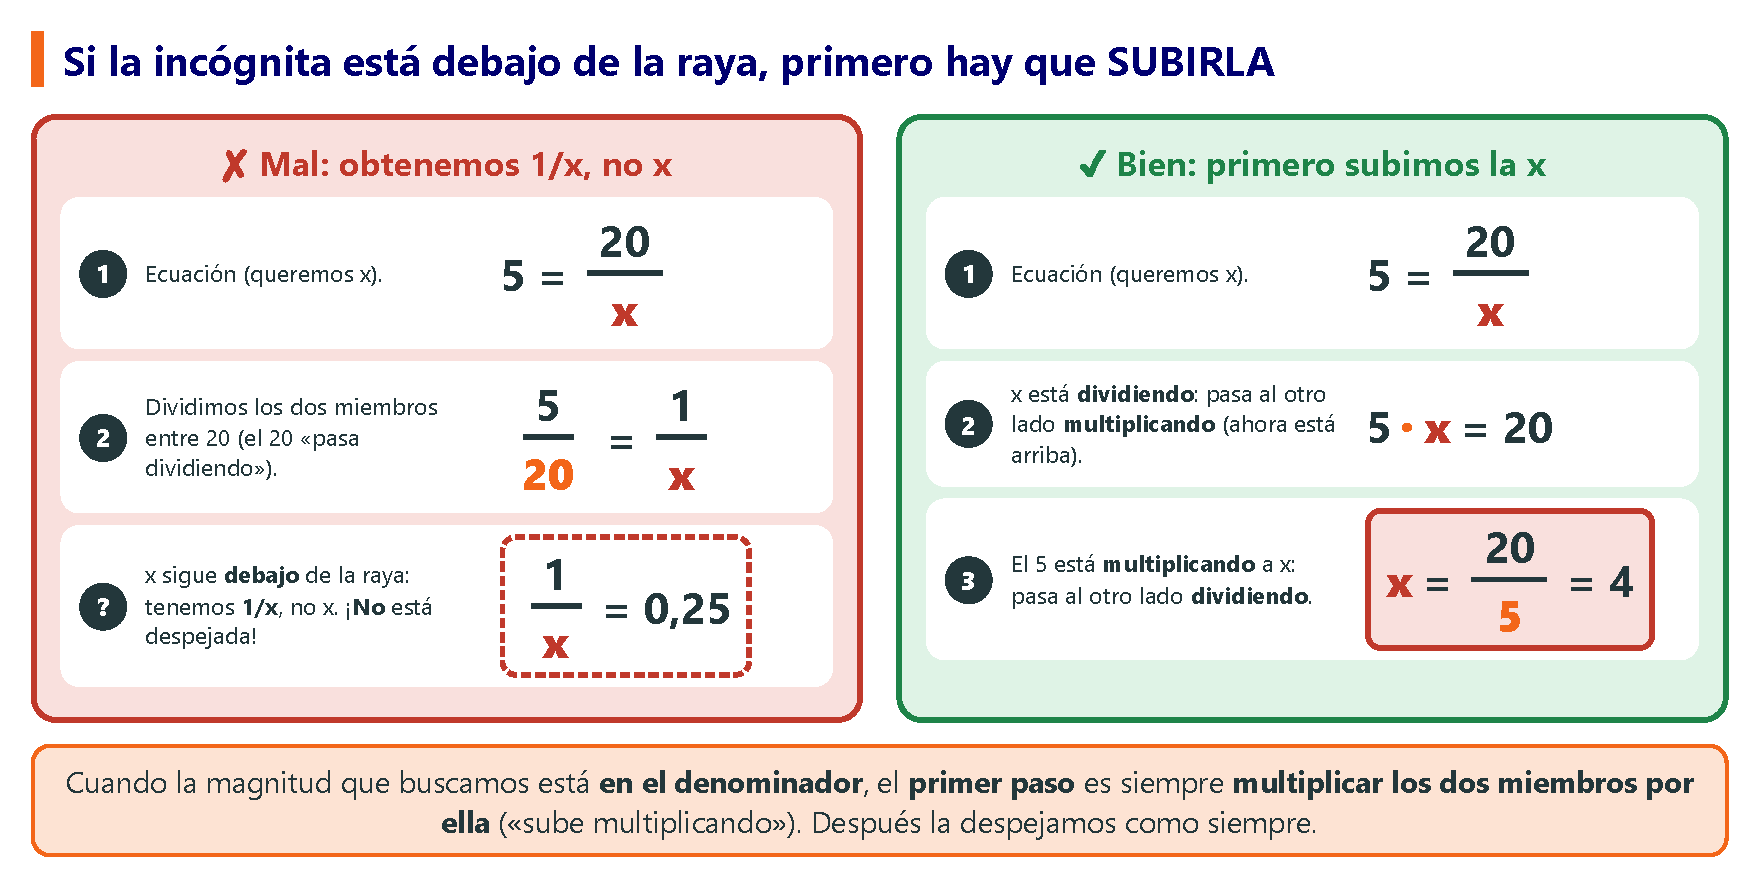
\includegraphics[width=\textwidth]{FigurasSVG/Unit_0_Math_Tools/pdf/denominator_up_es.pdf}
    \caption{Si la incógnita está en el denominador, primero hay que subirla (multiplicando); si no, obtenemos 1/x en lugar de x.}
    \label{fig:u0_denominator_up}
\end{figure}

\begin{example}
    \textbf{Despeja \(t\) en \(v = \dfrac{x}{t}\).}
    \begin{enumerate}[label=\numberballmDarkTeal]
        \item \(t\) está debajo de la raya, dividiendo: la subimos multiplicando (multiplicamos los dos miembros por \(t\)): \(v \cdot t = x\).
        \item Ahora \(v\) está multiplicando a \(t\): pasa al otro lado dividiendo: \(\textcolor{red}{t = \dfrac{x}{v}}\).
    \end{enumerate}
\end{example}

\begin{example}
    \textbf{Despeja \(V\) en \(d = \dfrac{m}{V}\) y calcúlalo para \(m = \qty{60}{\g}\) y \(d = \qty{3}{\g\per\cubic\cm}\).}
    \begin{enumerate}[label=\numberballmDarkTeal]
        \item \(V\) está debajo de la raya: sube multiplicando: \(d \cdot V = m\).
        \item \(d\) está multiplicando a \(V\): pasa al otro lado dividiendo: \(V = \dfrac{m}{d}\).
        \item \(V = \dfrac{\qty{60}{\g}}{\qty{3}{\g\per\cubic\cm}} = \textcolor{red}{\qty{20}{\cubic\cm}}\).
    \end{enumerate}
\end{example}

\subsection{Despejar en las fórmulas de física y química}

El método es exactamente el mismo con letras que con números. Estas son las fórmulas que más vas a usar este curso, con cada magnitud despejada:

\begin{table}[H]
    \centering
    \renewcommand{\arraystretch}{2.2}
    \begin{tabular}{llll}
        \toprule
        \textbf{Fórmula} & \multicolumn{3}{l}{\textbf{Magnitudes despejadas}} \\
        \midrule
         \(d = \dfrac{m}{V}\) & \(m = d \cdot V\) & \(V = \dfrac{m}{d}\) & \\
        \(v = \dfrac{x}{t}\) & \(x = v \cdot t\) & \(t = \dfrac{x}{v}\) & \\
        \(F = m \cdot a\) & \(m = \dfrac{F}{a}\) & \(a = \dfrac{F}{m}\) & \\
        \(W = m \cdot g\) & \(m = \dfrac{W}{g}\) & \(g = \dfrac{W}{m}\) & \\
        \(T = t_{\text{C}} + 273\) & \(t_{\text{C}} = T - 273\) & & \\
        \(p_1 \cdot V_1 = p_2 \cdot V_2\) & \(V_2 = \dfrac{p_1 \cdot V_1}{p_2}\) & \(p_2 = \dfrac{p_1 \cdot V_1}{V_2}\) & \\
        \bottomrule
    \end{tabular}
    \caption{Las fórmulas más habituales del curso, con cada magnitud despejada.}
    \label{tab:u0_formulas}
\end{table}

\begin{example}
    \textbf{Despeja \(v_f\) en \(a = \dfrac{v_f - v_i}{t}\).} Aquí la incógnita está dentro de una resta que está dividida entre \(t\):
    \begin{enumerate}[label=\numberballmDarkTeal]
        \item \(t\) está dividiendo a toda la resta: pasa al otro lado multiplicando: \(a \cdot t = v_f - v_i\).
        \item \(v_i\) está restando: pasa al otro lado sumando: \(\textcolor{red}{v_f = v_i + a \cdot t}\).
    \end{enumerate}
\end{example}

\begin{exercise}
    Despeja \(x\) usando \textbf{los dos} métodos y comprueba el resultado:
    \begin{enumerate}[label=\letraminuscula]
        \item \(x + 8 = 15\)
        \item \(x - 6 = 2\)
        \item \(5 \cdot x = 35\)
        \item \(\dfrac{x}{4} = 7\)
        \item \(3 \cdot x - 4 = 11\)
        \item \(\dfrac{x}{2} + 1 = 9\)
    \end{enumerate}
    \begin{solu}
        a) \(x = 15 - 8 = 7\); b) \(x = 2 + 6 = 8\); c) \(x = \dfrac{35}{5} = 7\); d) \(x = 7 \cdot 4 = 28\); e) \(3x = 11 + 4 = 15\), \(x = 5\); f) \(\dfrac{x}{2} = 9 - 1 = 8\), \(x = 16\).
    \end{solu}
\end{exercise}

\begin{exercise}
    La incógnita está en el denominador. Súbela primero y después despéjala:
    \begin{enumerate}[label=\letraminuscula]
        \item \(6 = \dfrac{30}{x}\)
        \item \(\dfrac{12}{x} = 4\)
        \item \(0{,}5 = \dfrac{2}{x}\)
        \item \(\dfrac{100}{x} = 25\)
    \end{enumerate}
    \begin{solu}
        a) \(6x = 30\), \(x = 5\); b) \(12 = 4x\), \(x = 3\); c) \(0{,}5x = 2\), \(x = 4\); d) \(100 = 25x\), \(x = 4\).
    \end{solu}
\end{exercise}

\begin{exercise}
    Despeja la magnitud que aparece entre paréntesis:
    \begin{enumerate}[label=\letraminuscula]
        \item \(d = \dfrac{m}{V}\) \quad (\(m\)) y (\(V\))
        \item \(v = \dfrac{x}{t}\) \quad (\(x\)) y (\(t\))
        \item \(F = m \cdot a\) \quad (\(a\))
        \item \(T = t_{\text{C}} + 273\) \quad (\(t_{\text{C}}\))
        \item \(\dfrac{V_1}{T_1} = \dfrac{V_2}{T_2}\) \quad (\(V_2\)) y (\(T_2\))
        \item \(a = \dfrac{v_f - v_i}{t}\) \quad (\(t\))
    \end{enumerate}
    \begin{solu}
        \begin{enumerate}[label=\alph*)]
            \item \(m = d \cdot V\); \(V = \dfrac{m}{d}\).
            \item \(x = v \cdot t\); \(t = \dfrac{x}{v}\).
            \item \(a = \dfrac{F}{m}\).
            \item \(t_{\text{C}} = T - 273\).
            \item \(V_2 = \dfrac{V_1 \cdot T_2}{T_1}\); \(T_2 = \dfrac{V_2 \cdot T_1}{V_1}\) (primero se multiplica en cruz: \(V_1 \cdot T_2 = V_2 \cdot T_1\)).
            \item \(t\) está en el denominador: \(a \cdot t = v_f - v_i\), así que \(t = \dfrac{v_f - v_i}{a}\).
        \end{enumerate}
    \end{solu}
\end{exercise}

\begin{exercise}
    Despeja la incógnita y calcula:
    \begin{enumerate}[label=\letraminuscula]
        \item La masa de una piedra con \(V = \qty{50}{\cubic\cm}\) y \(d = \qty{2.6}{\g\per\cubic\cm}\).
        \item El tiempo que tarda un coche que va a \(v = \qty{20}{\mps}\) en recorrer \(x = \qty{900}{\m}\).
        \item La aceleración de un carrito de \(\qty{40}{\kg}\) que se empuja con \(F = \qty{100}{\newton}\).
    \end{enumerate}
    \begin{solu}
        a) \(m = d \cdot V = \qty{2.6}{\g\per\cubic\cm} \cdot \qty{50}{\cubic\cm} = \qty{130}{\g}\); \quad
        b) \(t = \dfrac{x}{v} = \dfrac{\qty{900}{\m}}{\qty{20}{\mps}} = \qty{45}{\s}\); \quad
        c) \(a = \dfrac{F}{m} = \dfrac{\qty{100}{\newton}}{\qty{40}{\kg}} = \qty{2.5}{\mpss}\).
    \end{solu}
\end{exercise}

%----------------------------------------------------------------------------------------

\section{Gráficas}

\subsection{Los ejes de una gráfica}

Una gráfica tiene dos rectas perpendiculares, llamadas \textbf{ejes}, que se cortan en el \textbf{origen} (0, 0):
\begin{itemize}
    \item El \textbf{eje horizontal} (en matemáticas, el eje \(x\) o \textbf{eje de abscisas}).
    \item El \textbf{eje vertical} (en matemáticas, el eje \(y\) o \textbf{eje de ordenadas}).
\end{itemize}
Cada punto de la gráfica se escribe como \((\text{valor horizontal}, \text{valor vertical})\): el punto \((3, 5)\) está 3 unidades a la derecha y 5 unidades hacia arriba.

\begin{impt}
    \negsubro{En ciencias, los ejes no tienen por qué llamarse \(x\) e \(y\)}. Cada eje lleva el nombre (y la unidad) de la \textbf{magnitud} que representamos en él: \(t\) (s), \(v\) (m/s), \(m\) (g), \(T\) (\unit{\celsius})\ldots{} Cuando decimos «\textbf{A frente a B}» (en inglés, A \emph{vs} B), \textbf{A va en el eje vertical} y \textbf{B va en el eje horizontal}:
    \begin{itemize}
        \item «\(v\) frente a \(t\)»: \(v\) en el eje vertical y \(t\) en el eje horizontal.
        \item «\(x\) frente a \(t\)»: \(x\) en el eje vertical y \(t\) en el eje horizontal. Cuidado: ¡aquí la \(x\) va en el eje \textbf{vertical}!
        \item «\(m\) frente a \(V\)»: \(m\) en el eje vertical y \(V\) en el eje horizontal.
    \end{itemize}
    El tiempo va casi siempre en el eje \textbf{horizontal}.
\end{impt}

\begin{figure}[H]
    \centering
    % [FIGURA ORIGINAL] \includegraphics[width=\textwidth]{Unit_0/axes_names}
    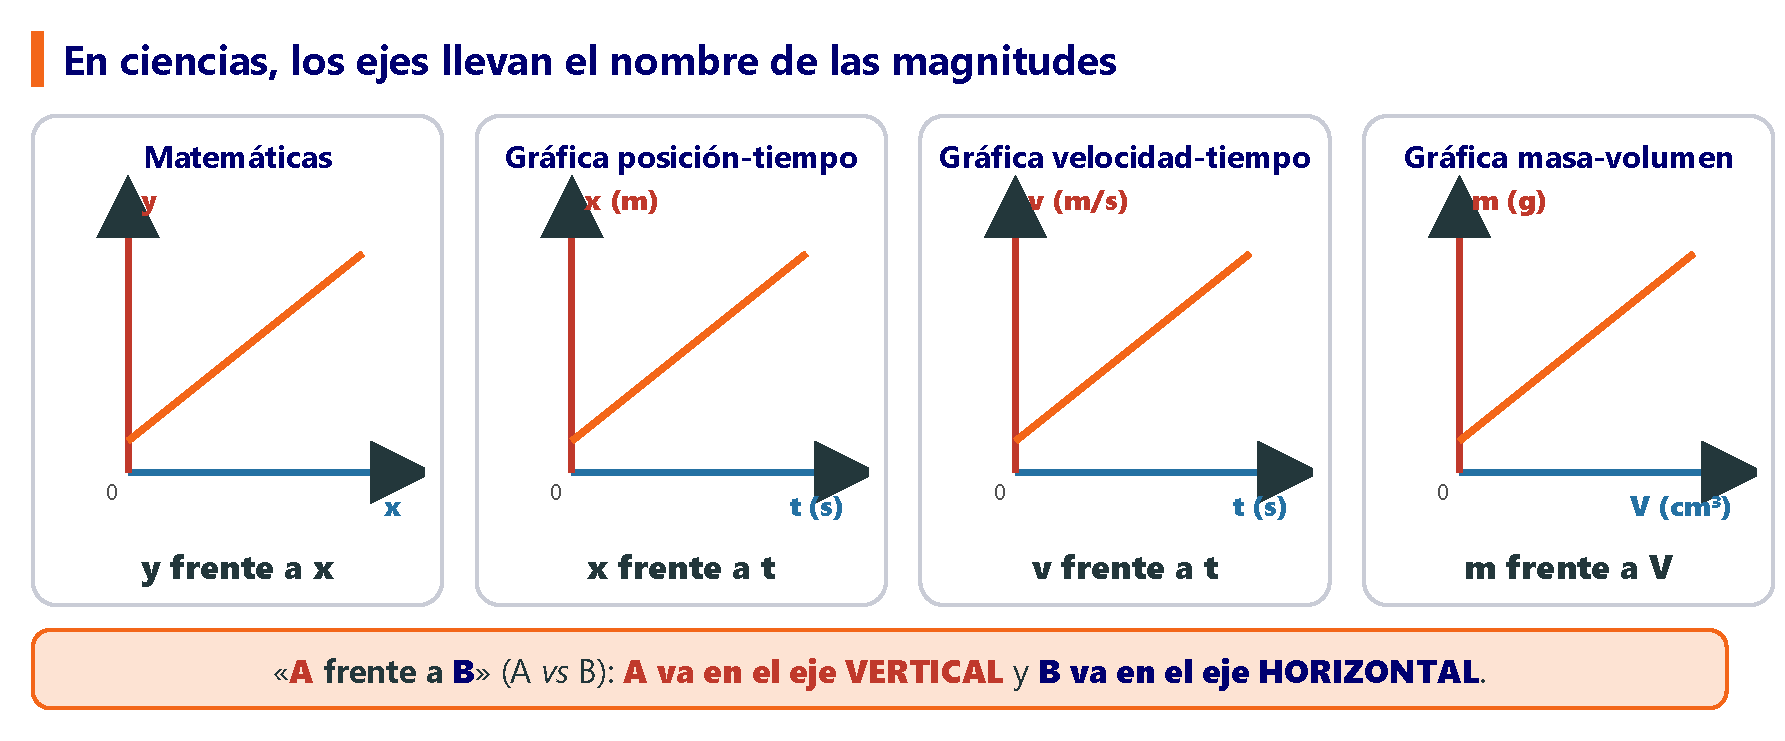
\includegraphics[width=\textwidth]{FigurasSVG/Unit_0_Math_Tools/pdf/axes_names_es.pdf}
    \caption{El mismo tipo de gráfica con los ejes nombrados según distintas magnitudes.}
    \label{fig:u0_axes_names}
\end{figure}

\subsection{Cómo dibujar una gráfica a partir de una tabla}

\negsubro{Método, paso a paso}:
\begin{enumerate}[label=\numberballmDarkTeal]
    \item Decide qué magnitud va en cada eje («A frente a B»: A en el vertical, B en el horizontal).
    \item Dibuja los ejes y \textbf{rotúlalos} con el nombre de la magnitud y su \textbf{unidad}.
    \item Elige una \textbf{escala} para cada eje, con divisiones iguales (por ejemplo, cada cuadrito son 2 s), de forma que quepan todos los valores de la tabla.
    \item Representa cada pareja de valores de la tabla como un \textbf{punto}.
    \item Si los puntos están en línea recta, únelos con una \textbf{regla}.
\end{enumerate}

\begin{example}
    \textbf{Matemáticas: dibuja la gráfica de \(y = 2x + 1\).} Primero hacemos una tabla, dando valores a \(x\):
    \begin{center}
        \begin{tabular}{lccccc}
            \toprule
            \(x\) & 0 & 1 & 2 & 3 & 4 \\
            \midrule
            \(y = 2x + 1\) & 1 & 3 & 5 & 7 & 9 \\
            \bottomrule
        \end{tabular}
    \end{center}
    \begin{center}
        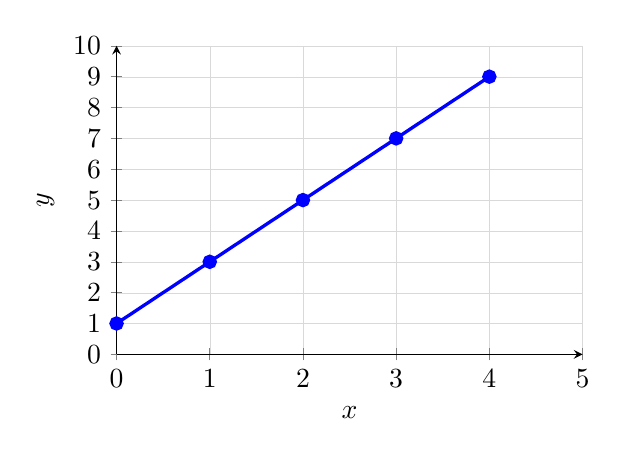
\begin{tikzpicture}
            \begin{axis}[width=7.5cm, height=5.5cm, grid=both, grid style={line width=.1pt, draw=gray!30},
                axis lines=left, xlabel={\(x\)}, ylabel={\(y\)}, xmin=0, xmax=5, ymin=0, ymax=10, xtick={0,1,...,5}, ytick={0,1,...,10}]
                \addplot[very thick, blue, mark=*] coordinates {(0,1) (1,3) (2,5) (3,7) (4,9)};
            \end{axis}
        \end{tikzpicture}
    \end{center}
\end{example}

\begin{example}
    \textbf{Ciencias: dibuja la gráfica \(m\) frente a \(V\) de varios trozos de aluminio.} Ahora los ejes se llaman \(m\) (vertical) y \(V\) (horizontal), y cada uno lleva su unidad:
    \begin{center}
        \begin{tabular}{lccccc}
            \toprule
            \(V\) (\unit{\cubic\cm}) & 0 & 10 & 20 & 30 & 40 \\
            \midrule
            \(m\) (\unit{\g}) & 0 & 27 & 54 & 81 & 108 \\
            \bottomrule
        \end{tabular}
    \end{center}
    \begin{center}
        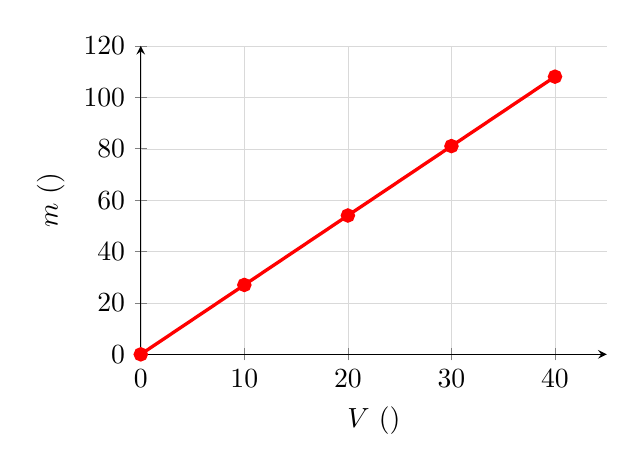
\begin{tikzpicture}
            \begin{axis}[width=7.5cm, height=5.5cm, grid=both, grid style={line width=.1pt, draw=gray!30},
                axis lines=left, xlabel={\(V\) (\unit{\cubic\cm})}, ylabel={\(m\) (\unit{\g})}, xmin=0, xmax=45, ymin=0, ymax=120, xtick={0,10,...,40}, ytick={0,20,...,120}]
                \addplot[very thick, red, mark=*] coordinates {(0,0) (10,27) (20,54) (30,81) (40,108)};
            \end{axis}
        \end{tikzpicture}
    \end{center}
    Es una recta que pasa por el origen: la masa y el volumen son \textbf{directamente proporcionales}.
\end{example}

\subsection{Análisis de gráficas de línea recta}

Para interpretar una gráfica de línea recta nos hacemos tres preguntas:

\begin{figure}[H]
    \centering
    % [FIGURA ORIGINAL] \includegraphics[width=\textwidth]{Unit_0/slope}
    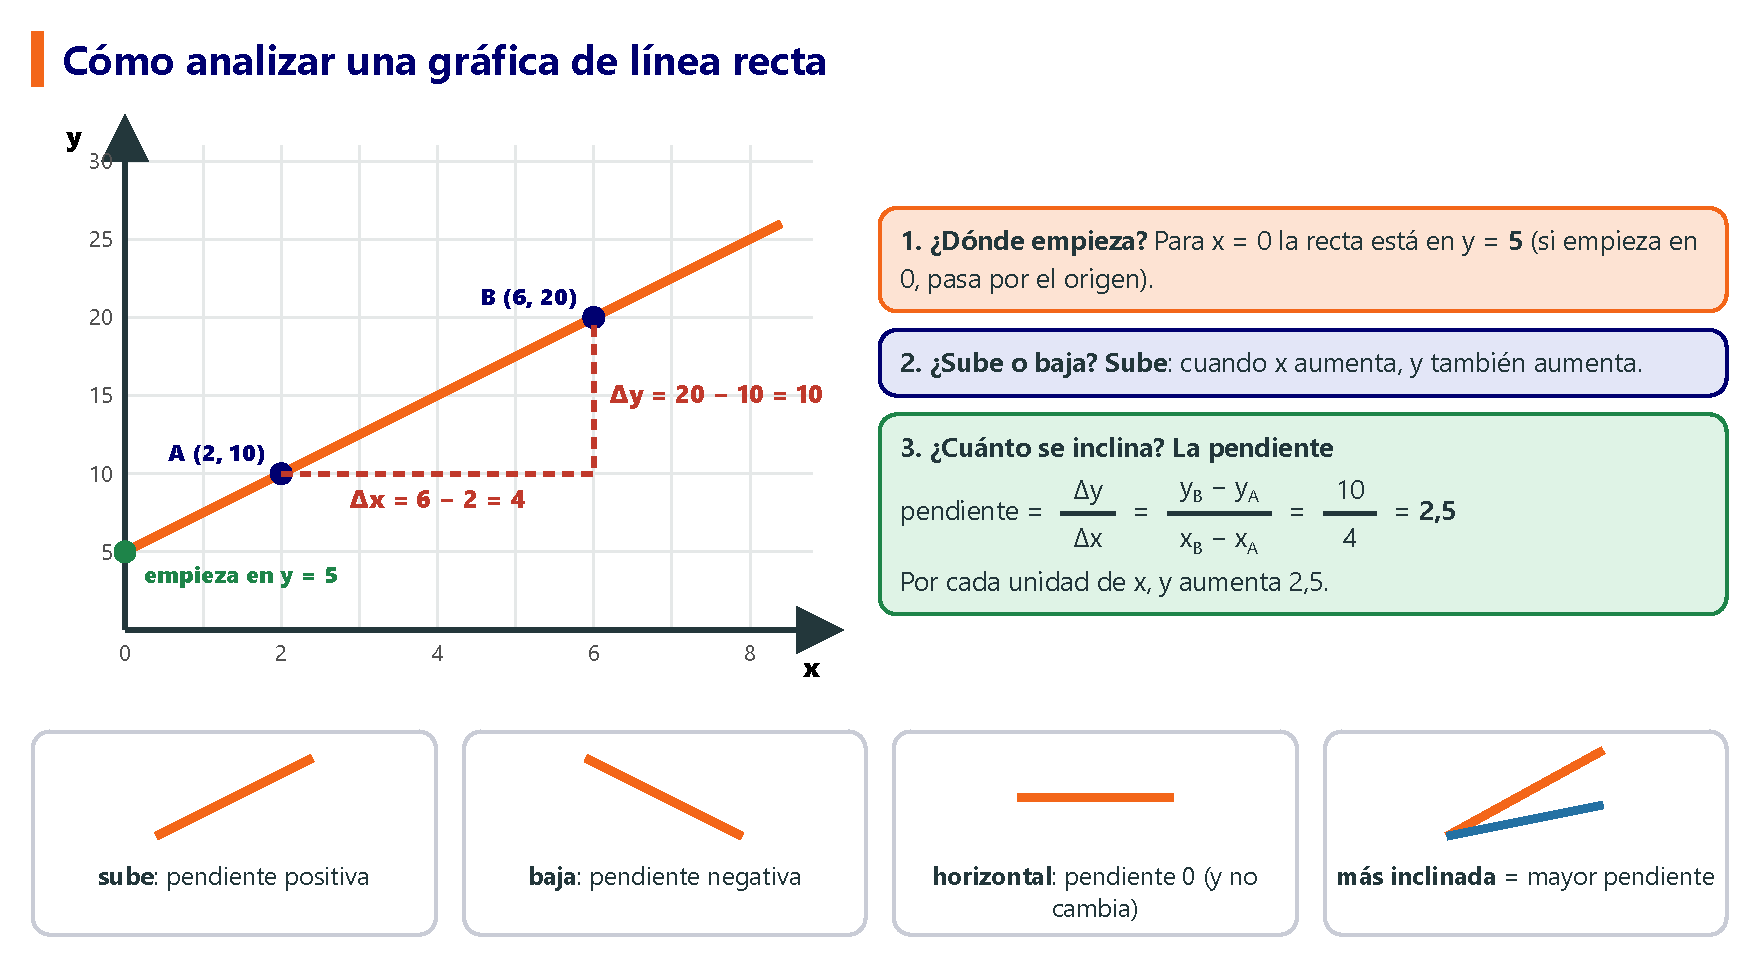
\includegraphics[width=\textwidth]{FigurasSVG/Unit_0_Math_Tools/pdf/slope_es.pdf}
    \caption{Dónde empieza, si sube o baja, y su pendiente.}
    \label{fig:u0_slope}
\end{figure}

\begin{enumerate}[label=\numberballmDarkTeal]
    \item \textbf{¿Dónde empieza?} Es el valor del eje vertical cuando el horizontal vale 0 (la \textbf{ordenada en el origen}). Si la recta pasa por \((0, 0)\), empieza en el \textbf{origen}.
    \item \textbf{¿Sube, baja o se mantiene horizontal?} Si sube, la magnitud del eje vertical \textbf{aumenta}; si baja, \textbf{disminuye}; si es horizontal, \textbf{no cambia}.
    \item \textbf{¿Cuánto se inclina?} Es la \negsubro{pendiente}: cuánto cambia la magnitud vertical por cada unidad de la horizontal. Tomamos dos puntos \(A\) y \(B\) de la recta:
    \begin{equation*}
        \text{pendiente} = \dfrac{\Delta(\text{vertical})}{\Delta(\text{horizontal})} = \dfrac{y_B - y_A}{x_B - x_A}
    \end{equation*}
\end{enumerate}

\begin{impt}
    \negsubro{En ciencias la pendiente tiene un significado}, y una unidad:
    \begin{itemize}
        \item Pendiente de una gráfica \(x\) frente a \(t\) \(= \dfrac{\Delta x}{\Delta t}\) = \textbf{velocidad} (\unit{\mps}).
        \item Pendiente de una gráfica \(v\) frente a \(t\) \(= \dfrac{\Delta v}{\Delta t}\) = \textbf{aceleración} (\unit{\mpss}).
        \item Pendiente de una gráfica \(m\) frente a \(V\) \(= \dfrac{\Delta m}{\Delta V}\) = \textbf{densidad} (\unit{\g\per\cubic\cm}).
    \end{itemize}
\end{impt}

\begin{example}
    \textbf{En la gráfica del aluminio de antes, calcula la pendiente y explica qué significa.} Tomamos \(A = (10, 27)\) y \(B = (30, 81)\):
    \begin{equation*}
        \text{pendiente} = \dfrac{\qty{81}{\g} - \qty{27}{\g}}{\qty{30}{\cubic\cm} - \qty{10}{\cubic\cm}} = \dfrac{\qty{54}{\g}}{\qty{20}{\cubic\cm}} = \textcolor{red}{\qty{2.7}{\g\per\cubic\cm}}
    \end{equation*}
    La pendiente de una gráfica \(m\) frente a \(V\) es la \textbf{densidad}: el aluminio tiene una densidad de \qty{2.7}{\g\per\cubic\cm}.
\end{example}

\begin{exercise}
    \textbf{Matemáticas.} Haz una tabla con \(x = 0, 1, 2, 3, 4\) y dibuja la gráfica de cada recta. Después di dónde empieza, si sube o baja, y calcula su pendiente:
    \begin{enumerate}[label=\letraminuscula]
        \item \(y = 3x\)
        \item \(y = x + 2\)
        \item \(y = 10 - 2x\)
    \end{enumerate}
    \begin{solu}
        \begin{enumerate}[label=\alph*)]
            \item Tabla: \(y = 0, 3, 6, 9, 12\). Empieza en el origen, sube, pendiente \(= \dfrac{12 - 0}{4 - 0} = 3\).
            \item Tabla: \(y = 2, 3, 4, 5, 6\). Empieza en \(y = 2\), sube, pendiente \(= \dfrac{6 - 2}{4 - 0} = 1\).
            \item Tabla: \(y = 10, 8, 6, 4, 2\). Empieza en \(y = 10\), baja, pendiente \(= \dfrac{2 - 10}{4 - 0} = -2\).
        \end{enumerate}
    \end{solu}
\end{exercise}

\begin{exercise}
    \textbf{Ciencias.} Calentamos una olla con agua y medimos su temperatura cada minuto:
    \begin{center}
        \begin{tabular}{lcccccc}
            \toprule
            \(t\) (min) & 0 & 1 & 2 & 3 & 4 & 5 \\
            \midrule
            \(T\) (\unit{\celsius}) & 20 & 30 & 40 & 50 & 60 & 70 \\
            \bottomrule
        \end{tabular}
    \end{center}
    \begin{enumerate}[label=\letraminuscula]
        \item Dibuja la gráfica «\(T\) frente a \(t\)». ¿Qué magnitud va en cada eje?
        \item ¿Cuál es la temperatura inicial?
        \item Calcula la pendiente. ¿Qué significa?
    \end{enumerate}
    \begin{solu}
        \begin{enumerate}[label=\alph*)]
            \item \(T\) en el eje vertical y \(t\) en el eje horizontal. Los puntos forman una recta que sube.
            \item \qty{20}{\celsius} (el valor para \(t = 0\)).
            \item Pendiente \(= \dfrac{\qty{70}{\celsius} - \qty{20}{\celsius}}{\qty{5}{\minute} - \qty{0}{\minute}} = \qty{10}{\celsius}\) por minuto: la temperatura sube \qty{10}{\celsius} cada minuto.
        \end{enumerate}
    \end{solu}
\end{exercise}

\begin{exercise}
    Observa la gráfica «\(v\) frente a \(t\)» de un coche y responde a las preguntas.
    \begin{center}
        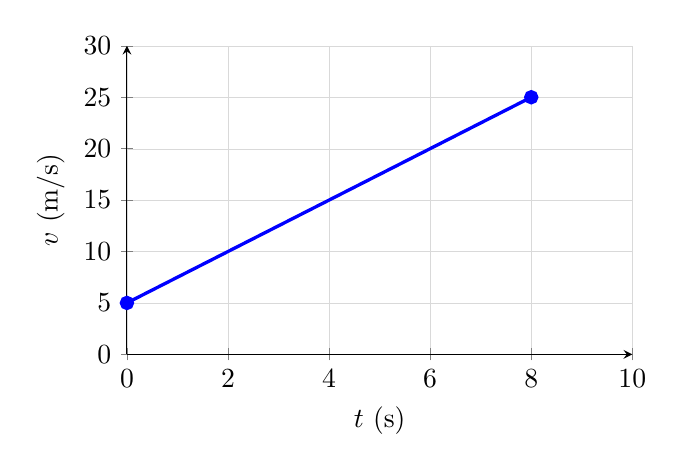
\begin{tikzpicture}
            \begin{axis}[width=8cm, height=5.5cm, grid=both, grid style={line width=.1pt, draw=gray!30},
                axis lines=left, xlabel={\(t\) (s)}, ylabel={\(v\) (m/s)}, xmin=0, xmax=10, ymin=0, ymax=30, xtick={0,2,...,10}, ytick={0,5,...,30}]
                \addplot[very thick, blue, mark=*] coordinates {(0,5) (8,25)};
            \end{axis}
        \end{tikzpicture}
    \end{center}
    \begin{enumerate}[label=\letraminuscula]
        \item ¿Qué magnitud hay en cada eje?
        \item ¿Cuál es la velocidad en \(t = 0\)? ¿Y en \(t = \qty{4}{\s}\)?
        \item ¿La velocidad aumenta o disminuye?
        \item Calcula la pendiente. ¿Qué magnitud es?
    \end{enumerate}
    \begin{solu}
        \begin{enumerate}[label=\alph*)]
            \item \(v\) (m/s) en el eje vertical y \(t\) (s) en el eje horizontal.
            \item En \(t = 0\): \(v = \qty{5}{\mps}\). En \(t = \qty{4}{\s}\): \(v = \qty{15}{\mps}\).
            \item Aumenta: la recta sube.
            \item Pendiente \(= \dfrac{\qty{25}{\mps} - \qty{5}{\mps}}{\qty{8}{\s} - \qty{0}{\s}} = \qty{2.5}{\mpss}\). Es la \textbf{aceleración}.
        \end{enumerate}
    \end{solu}
\end{exercise}

\begin{exercise}
    Dibuja en los mismos ejes las gráficas «\(x\) frente a \(t\)» de dos ciclistas, usando estas tablas. ¿Quién va más rápido? ¿Cómo se ve en la gráfica?
    \begin{center}
        \begin{tabular}{lccccc}
            \toprule
            \(t\) (s) & 0 & 2 & 4 & 6 & 8 \\
            \midrule
            \(x_A\) (m) & 0 & 8 & 16 & 24 & 32 \\
            \(x_B\) (m) & 0 & 12 & 24 & 36 & 48 \\
            \bottomrule
        \end{tabular}
    \end{center}
    \begin{solu}
        Las dos son rectas que pasan por el origen. Pendiente de \(A\): \(\dfrac{32}{8} = \qty{4}{\mps}\); pendiente de \(B\): \(\dfrac{48}{8} = \qty{6}{\mps}\). \(B\) va más rápido: su recta está \textbf{más inclinada} (tiene mayor pendiente).
    \end{solu}
\end{exercise}

%----------------------------------------------------------------------------------------

\section*{Resumen}

\begin{itemize}
    \item \textbf{Potencias de 10}: \(10^{n}\) es un 1 seguido de \(n\) ceros; \(10^{-n}\) tiene el 1 en el lugar \(n\) después de la coma; \(10^{0} = 1\).
    \item \textbf{Reglas}: \(10^{a} \cdot 10^{b} = 10^{a+b}\); \(\dfrac{10^{a}}{10^{b}} = 10^{a-b}\); \(\dfrac{1}{10^{b}} = 10^{-b}\) (una potencia de 10 cambia el signo de su exponente al cruzar la raya de fracción); \(\left(10^{a}\right)^{b} = 10^{a \cdot b}\).
    \item \textbf{Despejar} una magnitud es dejarla sola, en el numerador, en un lado de la ecuación. Hacemos la operación contraria en los dos miembros o, con el atajo, la pasamos al otro lado con la operación contraria.
    \item Si la incógnita está en el \textbf{denominador}, primero la subimos multiplicando; si no, obtenemos \(1/x\), no \(x\).
    \item \textbf{Gráficas}: «A frente a B» significa A en el eje vertical y B en el eje horizontal. Una gráfica de línea recta se describe por dónde empieza, si sube o baja, y su \textbf{pendiente} \(= \Delta(\text{vertical}) / \Delta(\text{horizontal})\).
\end{itemize}
